%第3章

\section{要求定義}

感染症予防サポートシステムがどのような機能を持ち,どのような振る舞いをするかを表すために以下の図\ref{usecase1}に示すユースケース図を作成した.

\begin{figure}[htbp]
\centering
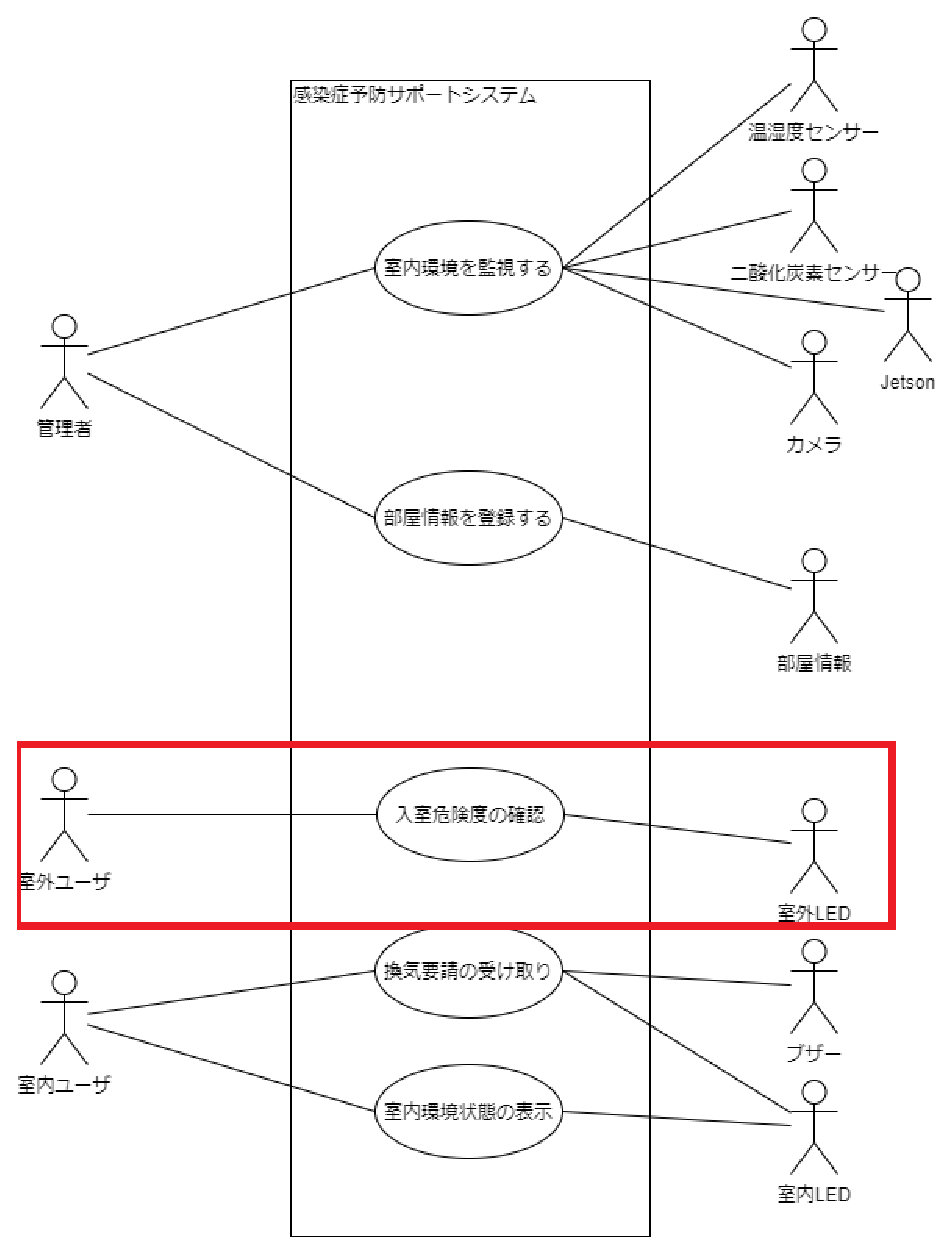
\includegraphics[width = 10cm]{./uml/usecase_e.eps}
\caption{ユースケース図}
\label{usecase1}
\end{figure}

感染症予防サポートシステムの各ユースケースについて述べる.
「室内環境を監視する」では,Webカメラにより取得した画像について人数推定を行い,室内人数に応じた監視モードを開始する.監視モードで測定した二酸化炭素濃度に応じて警戒レベルを設定し,必要に応じて換気要請を出すなどの対応をとる.
「部屋情報を登録する」では,管理者が登録した,システムを運用する部屋の広さを元に,標準警戒レベルでの滞在可能上限人数を定める.
「入室危険度の確認」では,部屋の滞在可能上限人数と現在の室内人数に応じた入室危険度を表す室外デバイスのLEDを点灯する.
「換気要請の受け取り」では,二酸化炭素濃度が各警戒レベルでの基準値を一定時間連続で超えると,LEDやブザーによって換気要請が出され,室内のユーザーは要請に従い換気を行う.
「室内環境状態の表示」では,温湿度の一定時間ごとの測定値を元に室内環境を分析し,温湿度が基準値を超えている場合は室内のLEDが点灯する.これを受けた室内のユーザーは,エアコン等により温湿度の調整を行う.
特に赤枠で囲んだ「入室危険度の確認」は筆者が実装を担当する部分となる.

上記のユースケースを受け,表\ref{sougoutestkoumoku}に示す総合テストの項目を挙げた.

\begin{table}
	\centering
	\caption{総合テスト項目}
	\label{sougoutestkoumoku}
	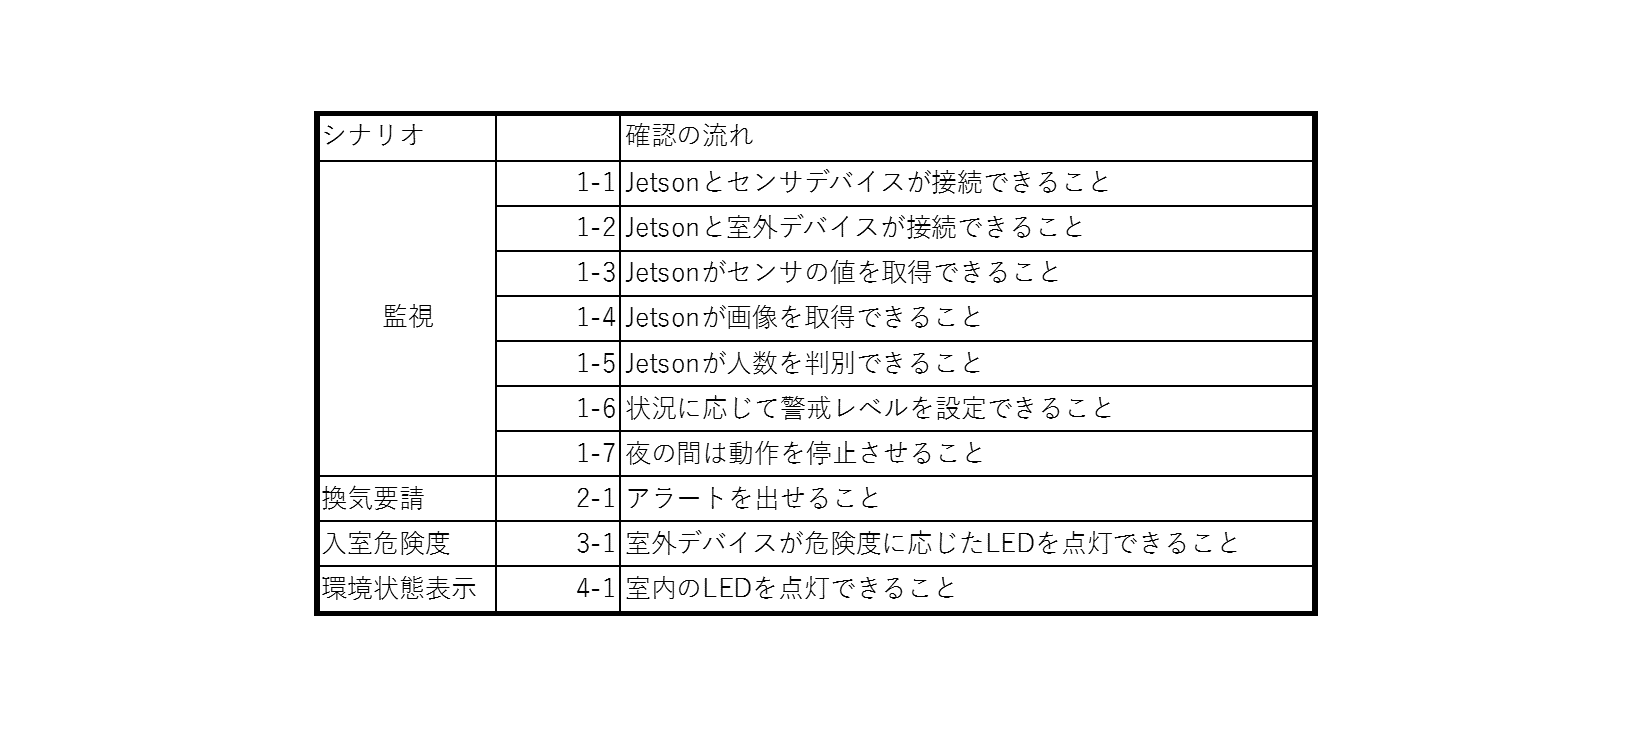
\includegraphics[width=0.9\linewidth]{test/sougoutest_koumoku}
\end{table}
\newpage